\documentclass[a4paper,12pt, oneside]{book}

%\usepackage{fullpage}
\usepackage[T1]{fontenc}
\usepackage[italian]{babel}
\usepackage[utf8]{inputenc}
\usepackage{amssymb}
\usepackage{amsthm}
\usepackage{graphics}
\usepackage{amsfonts}
\usepackage{listings}
\usepackage{amsmath}
\usepackage{amstext}
\usepackage{engrec}
\usepackage{rotating}
\usepackage[safe,extra]{tipa}
\usepackage{showkeys}
\usepackage{multirow}
\usepackage{hyperref}
\usepackage{microtype}
\usepackage{enumerate}
\usepackage{braket}
\usepackage{marginnote}
\usepackage{pgfplots}
\usepackage{cancel}
\usepackage{polynom}
\usepackage{booktabs}
\usepackage{enumitem}
\usepackage{framed}
\usepackage{pdfpages}
\usepackage{pgfplots}
\usepackage[usenames,dvipsnames]{pstricks}
\usepackage{epsfig}
\usepackage{pst-grad} % For gradients
\usepackage{pst-plot} % For axes
\usepackage[space]{grffile} % For spaces in paths
\usepackage{etoolbox} % For spaces in paths
\makeatletter % For spaces in paths
\patchcmd\Gread@eps{\@inputcheck#1 }{\@inputcheck"#1"\relax}{}{}
\makeatother
\usepackage[cache=false]{minted}
\usepackage{fancyhdr}
\newcommand{\numberset}{\mathbb}
\newcommand{\N}{\numberset{N}}
\newcommand{\Z}{\numberset{Z}}
\newcommand{\Q}{\numberset{Q}}
\newcommand{\R}{\numberset{R}}

\pagestyle{fancy}
\fancyhead[LE,RO]{\slshape \rightmark}
\fancyhead[LO,RE]{\slshape \leftmark}
\fancyfoot[C]{\thepage}



\title{Probabilità e Statistica per l'Informatica}
\author{UniShare\\\\Davide Cozzi\\\href{https://t.me/dlcgold}{@dlcgold}\\\\Gabriele De Rosa\\\href{https://t.me/derogab}{@derogab} \\\\Federica Di Lauro\\\href{https://t.me/f_dila}{@f\textunderscore dila}}
\date{}

\pgfplotsset{compat=1.13}
\begin{document}
\maketitle
\tableofcontents

\definecolor{shadecolor}{gray}{0.80}

\newtheorem{teorema}{Teorema}
\newtheorem{definizione}{Definizione}
\newtheorem{esempio}{Esempio}
\newtheorem{corollario}{Corollario}
\newtheorem{lemma}{Lemma}
\newtheorem{osservazione}{Osservazione}
\newtheorem{nota}{Nota}
\newtheorem{esercizio}{Esercizio}
\newcommand{\mean}[1]{\overline #1}
\renewcommand{\chaptermark}[1]{%
\markboth{\chaptername
\ \thechapter.\ #1}{}}
\renewcommand{\sectionmark}[1]{\markright{\thesection.\ #1}}
\chapter{Introduzione}
\textbf{Questi appunti sono presi a lezione. Per quanto sia stata fatta una revisione è altamente probabile (praticamente certo) che possano contenere errori, sia di stampa che di vero e proprio contenuto. Per eventuali proposte di correzione effettuare una pull request. Link: } \url{https://github.com/dlcgold/Appunti}.\\
\textbf{Grazie mille e buono studio!}
\chapter{Breve Introduzione}
La statistica è una discliplina, basata sulla matematica, con il fine lo studio quantitativo e qualitativo
di un particolare fenomeno collettivo in condizioni di incertezza o non determinismo ed è usata in molti 
ambiti come ad esempio l'intelligenza artificiale, data science, robotica, domotica e tutte le analisi 
per poter ottenere ricavare delle informazioni sui dati.

Ormai i dati sono pervasivi e un loro studio è diventato necessario ed inoltre si parla spesso di target marketing,
con una selezione dei possibili clienti infatti è usata in maniera massiccia nel mondo dello shopping online.\newline
Si ha l'\textit{A-B testing}, per decidere tra due scelte la migliore e per la decisione si analizzano i dati
presi da campioni di popolazione, utilizzando il \textit{tasso di conversione}, ossia la percentuale di visitatori unici
che hanno effettuato la azione su cui si sta effettuando il test.

In codesto corso vengono effettuati i seguenti argomenti:
\begin{enumerate}
    \item statistica descrittiva
    \item calcolo delle probabilità
    \item distribuzioni notevoli
    \item teoremi di convergenza
    \item stima dei parametri
    \item test di ipotesi parametrici
    \item test di ipotesi non parametrici
    \item regressione lineare
\end{enumerate}

\chapter{Statistica Descrittiva}
La statistica descrittiva è una raccolta di metodi e strumenti matematici usati per organizzare una o più serie di dati
al fine di trovarne delle simmetrie, periodicità o delle eventuali leggi, ossia si effettua una descrizione 
delle informazioni implicite ai dati.

Solitamente i dati disponibili non rappresentano tutta la popolazione ma un numero limitato 
di osservazioni effettuato su un \emph{campione}, sottoinsieme selezionato della popolazione su cui si effettua
l'analisi statistica, la cui efficacia rispetto alla popolazione dipende da quale sottoinsieme è stato scelto
infatti non esiste un solo campione ma vi sono diversi modi per sceglierli, più o meno efficaci, per l'analisi statistica.

Quando si effettua un analisi statistica si vuole affermare qualcosa riguardo i \textbf{caratteri} della popolazione,
ossia gli elementi su cui effettuo l'analisi statistica, che possono essere:
\begin{itemize}
    \item \textbf{caratteri qualitativi}, indicanti qualità (colori, stili, materiali etc...) e anche dati non numerici
             in cui solitamente non è definita una \textit{relazione d'ordine}
    \item \textbf{caratteri quantitativi}, maggiormente studiati dal corso, dati numerici in cui vengono definite \emph{relazioni d'ordine}:
        \begin{itemize}
            \item \textbf{discreti}, come i lanci di un dado, rappresentanti valori in $\Z$
            \item \textbf{continui}, che assumono valori reali, come la temperatura, in $\R$
        \end{itemize}
\end{itemize}
Supponiamo di considerare $n$ elementi della popolazione e di rilevare, per ognuno di essi,
il dato relativo al carattere quantitativo da esaminare, ossia definiamo l'insieme di dati
$E=\{x_1, x_2, \dots, x_n\}$ con la numerosità, il numero di elementi considerati, pari a $n$.

In caso il carattere è quantitativo discreto è comodo raggruppare i dati considerando 
l'insieme di tutti i valori assumibili, detta \textbf{modalità del carattere} ed associare ad ognuno 
di esso il numero di volte che esso compare in $E$.\newline
Si ha quindi $N$ il numero di totalità del carattere e si definisce l'insieme di modalita
$S=\{s_1,...,s_N\}$ su cui si definiscono i seguenti valori statistici:
\begin{description}
    \item [frequenza assoluta $f_j$] numero di volte che si presenta un elemento di un campione
    \item [frequenza cumulata assoluta $F_j$] somma delle frequenze assolute di tutte le modalità:
            \[ F_j = \sum_{k:s_k \leq s_j} f_k \]
    \item [frequenza relativa $p_j$] rapporto tra la frequenza assoluta e il numero di elementi 
            \[ p_j = \frac{f_j}{n} \]
    \item [frequenza cumulativa relativa $P_j$] somma delle frequenze relativa di tutte le modalità:
            \[ P_j = \sum{k:s_k \leq s_j} p_k \]
\end{description}
Si definisce \textbf{distribuzione di frequenza} una funzione $F:S \to \N$ che associa ad ogni modalità la corrispondente frequenza
per cui esiste la distribuzione di frequenza assoluta, relativa, frequenza cumulativa assoluta e relativa.

%inserire esempio pagina 9
Quando il carattere da studiare è continuo (o discreto con un gran numero di valori) è conveniente 
ricondursi a raggruppamenti come quelli appena trattati, per cui si suddivide $S$, l'insieme delle modalità,
in alcune classi (sottoinsiemi di $S$) che formano una partizione e la scelta delle classi con cui 
si suddivide l'insieme $S$ è del tutto arbitraria anche se è necessario che esse formino una partizione di $S$.\newline
Le partizioni devono essere significative e sufficientemente numerose ed inoltre ad ogni classe si associano le grandezze:
\begin{itemize}
\item confine superiore e inferiore (valori estremi della classe)
\item ampiezza (differenza tra confine superiore ed inferiore)
\item valore centrale (media tra i due confini)
\end{itemize}
Nel caso in cui il carattere esaminato sia continuo occorre specificare come le classi sono chiuse, a destra o a sinistra,
ossia specificare se gli elementi dell'indagine il cui dato coincide con il confine della classe sono da raggruppare
all'interno della classe stessa oppure no.
%esempio a pagina 13
\section{Indici di tendenza Generale}
Fino ad ora abbiamo visto come rappresentare i dati, sia discreti che continui, ora iniziamo ad analizzare gli indici
che ci forniscono un valore che rappresenta un certo aspetto della serie di dati, 
incominciando dagli \textbf{indici di tendenza generale}:
\begin{description}
    \item [media] è la media aritmetica tra tutti i valori dei dati osservati 
            \[ \overline{x} = \frac{1}{n} \sum x_i = \frac{x_1 + \cdots + x_n}{n} \]
            Considerando le distribuzioni di frequenza definite, posssiamo fornire definizioni equivalenti di media:
                \[ \overline{x} = \frac{1}{n} \sum s_j f_j = \sum s_j p_j \]
                La dimostrazione dell'uguaglianza di queste definizioni alternative è banale e si riconduce 
                alla definizione di frequenza relativa ed assoluta.

    \item [mediana] è l'elemento in mezzo ai valori dei dati, ordinati in maniera crescente
            in cui se il numero degli elementi $n$ è dispari è l'elemento $\frac{n + 1}{2}$
            altrimenti è la somma degli elementi di posto $\frac{n}{2}$ e $\frac{n}{2} + 1$.

    \item [moda $\widetilde{x}$] valore o classe corrispondente alla massima frequenza assoluta e viene usata 
            solitamente in caso sia impossibile definire la media e la mediana.\newline
            La moda non è unica infatti parliamo di:
            \begin{itemize}
                 \item \textbf{distribuzione uni-modale} nel caso in cui vi sia un unica moda
                 \item \textbf{distribuzione multi-modale} nel caso in cui vi siano più mode
            \end{itemize}
\end{description}
%aggiungo esempio
Gli indici di tendenza centrale non sono utili per fornire informazioni circa l'omogeneità dei dati in quanto forniscono 
informazioni sui valori centrali e medi del campione statistico per cui per risolvere sto problema introduciamo i seguenti indici:
\begin{description}
        \item [varianza] è la media dello scarto quadratico di ogni elemento dalla sua media 
                \[ s^2 = \frac{1}{n} \sum _{i = 1} ^ n (x_i - \overline{x})^2 \]
                La varianza ovviamente è tanto più grande quanto i singoli elementi si discostano dalla media, 
                ossia significa che i dati in tal caso sono molto disomogenei.
                Come abbiamo già visto per la media sono presenti le seguenti definizioni alternative di varianza:
                \[ s^2 = \frac{1}{n} \sum _{j = 1} ^ N f_j (s_j - \overline{x}) ^ 2 \]
                \[ s^2 = \sum _{j = 1} ^ N p_j (s_j - \overline{x}) ^ 2 \]
                \[ s^2 = \sum _{j = 1} ^ n x_j - \overline{x} ^ 2 \]
                Le prime due definizioni alternative derivano dalla definizione di frequenza assoluta e frequenza 
                mentre l'ultima proviene da passaggi algebrici, dimostrati di seguito formalmente:
                \begin{proof}
                        \[ \begin{split}
                            s^2 & = \frac{1}{n} \sum _{i = 1} ^ n (x_i - \mean{x}) ^ 2 \\
                                & = \frac{1}{n} \sum (x_i ^ 2 - 2x_i\mean{x} + \mean{x} ^ 2) \\
                                & = \frac{1}{n} (\sum x_i^2 - 2\mean{x} \sum x_i + \sum \mean{x} ^ 2) \\
                                & = \frac{1}{n} (\sum x_i^2 - 2n\mean{x}^2 + n\mean{x}^2) \\
                                & = \frac{1}{n} \sum x_i^2 - \mean{x} ^ 2 \\
                            \end{split} \]
                Si dimostra $\sum x_i = n \mean{x}$ in quanto $\mean{x} = \frac{1}{n} \sum x_i$ e il resto 
                sono soltanto passaggi algebrici elementari
                \end{proof}

    \item [scarto quadratico medio] misura quanto sono distanti gli elementi di un campione ed è calcolata come:
            \[ s = \sqrt{s^2} = \sqrt{\frac{1}{n} \sum _{i = 1} ^ n (x_i - \overline{x}) ^ 2} \]
\end{description}
Nel calcolo della varianza si utilizza il quadrato per la differenza tra l'elemento e la sua media in quanto 
per come è definita la media si ha $\sum (x_i - \overline{x}) = 0$ e per evitare ciò si eleva la differenza 
tra un elemento e la sua media al quadrato.

La varianza è definito come il momento secondo rispetto alla media, espresso tramite la formula:
\[ M_{k,y}=\frac{1}{n}\sum (x_i-y)^2 \]

\section{Il caso bidimensionale}
Fino ad ora noi abbiamo considerato il caso unidimensionale in cui consideriamo solo un carattere del campione ma 
molte analisi richiedono di analizzare due o più caratteri del campione contemporaneamente, per riconoscere 
leggi ed analogie tra i diversi caratteri.\newline
Considereremo solo due caratteri contemporanei, sia perché un analisi con più caratteri si comporta uguale e sia 
per non aggravare troppo la rappresentazione dei dati negli esempi e assumiamo che entrambi i caratteri sono di
tipo quantitativo e discreto, in quanto se fossero quantitativi continui subirebbero prima un raggruppamento a classi.

L'insieme dei dati viene rappresentato come l'insieme delle coppie
\[ E = \{(x_1, y_1), (x_2, y_2) \dots, (x_n, y_n)\} \]
mentre l'insieme delle coppie di valori assumibili si rappresentati con l'insieme
\[ S = \{(s_j, u_k), \, j = 1 \dots N \quad k = 1 \dots M\} \]
Come abbiamo fatto anche per il caso unidimensionale definiamo le seguenti quantità:
\begin{description}
    \item [frequenza assoluta $(s_j, u_k)$] è la quantita $f_{jk}$ corrispondente al numero di elementi con valore $(s_j, u_k)$
    \item [frequenza relativa] \[ p_{jk} = \frac{f_{jk}}{n} \] rapporto tra la frequenza e il numero di elementi
    \item [frequenza cumulata assoluta]  \[ F_{jk} = \sum _{r:s_r \leq s_j; l:u_l \leq u_k} f_{rl} \]
    \item [frequenza cumulata relativa] \[ P_{jk} = \sum _{r:s_r \leq s_j; u_l \leq u_k} p_{rl} \] frequenza 
\end{description}
Si definisce \emph{distribuzione di frequenza doppia} una qualsiasi funzione $f, F, p, P$ 
che associa ad ogni coppia $(s_j, u_k)$ la corrispondente frequenza ma esistono anche altri tipi di distribuzioni,
infatti noi vediamo le \textbf{distribuzioni marginali}: distribuzioni dei singoli caratteri presi indipendemente degli altri.

Le distribuzioni marginali hanno la definizione delle seguenti funzioni:
\begin{description}
    \item [frequenza assoluta marginale] quantità di elementi $f_xj$ data dagli elementi di $E$, il cui primo carattere ha valore $s_j$
    \item [frequenza relativa marginale] rapporto tra la frequenza assoluta marginale e il numero di osservazioni $n$.
    \item [frequenza cumulata assoluta marginale] $F_{xj}$ somma delle frequenze assolute marginali di tutti gli $s_k$ con $s_k \leq s_j$
    \item [frequenza cumulata relativa marginale] $P_{xj}$ somma delle frequenze relative marginali di tutti gli $s_k$ con $s_k \leq s_j$
\end{description}
Oltre agli indici definiti fino ad ora, esiste un indice che fornisce un grado di interdipendenza tra i due caratteri,
indice importante in quanto molti problemi concreti necessitano di analizzare gradi di correlazione tra due o più serie di dati,
iniziando prima di tutto da un esempio.

Considero due serie $\{x_i\},\{y_i\},\,\,i=1,...,n$ ponendo a confronto le variazione delle coppie di dati
rispetto ai corrispondenti valori medi, considerando le coppie di scarti:
\[ x_i - \overline{x} \]
\[ y_i - \overline{y} \]
si ha una relazione di dipendenza tra i due caratteri se i due scarti corrispondono sistematicamente o quasi valori positivi o negativi.

Si definisce quindi la \textbf{covarianza} $c_{xy}$, dei dati o campionaria, delle due serie di dati :
\[ c_{xy} = \frac{1}{n} \sum (x_i - \overline{x}) (y_i - \overline{y}) \]
La covarianza assume un valore positivo (negativo) che diviene grande in valore assoluto nel caso in cui 
i termini prodotto abbiano segni concordi e in questo caso si parla di serie statistiche fortemente correlate
o per meglio dire di dati delle serie fortemente correlati.\newline
Nel caso opposto vale a dire nel caso in cui i dati delle serie siano incorrelati avremo che i prodotti
avranno segni diversi (saranno discordi in segno) e la covarianza, per come definita,
risulterà piccola in valore assoluto, prossima al valore 0.

Si ha anche la seguente formula per la covarianza:
\[ c_{xy} = \frac{1}{n} \sum x_iy_i - \overline{x}\overline{y} \]
\begin{proof}
        \[ \begin{split}
                c_{xy} & = \frac{1}{n} \sum _{i = 1} ^ n (x_i - \mean{x}) (y_i - \mean{y}) \\
                       & = \frac{1}{n} \sum _{i = 1} ^ n (x_iy_i - x_i\mean{y} - y_i \mean{x} + \mean{x}\mean{y}) \\
                       & = \frac{1}{n} (\sum x_iy_i - \mean{y} \sum x_i - \mean{x} \sum y_i + \sum \mean{x}\mean{y}) \\
                       & = \frac{1}{n} (\sum x_iy_i - n\mean{y}\mean{x} - n\mean{y}\mean{x} + n\mean{y}\mean{x}) \\
                       & = \frac{1}{n} (\sum x_iy_i - n\mean{x}\mean{y}) \\
                       & = \frac{1}{n} \sum x_iy_i - \mean{x}\mean{y} \\
            \end{split} \]
\end{proof}
Nel caso in cui i dati si riferiscano a caratteri quantitativi discreti, di cui è nota la
distribuzione di frequenza doppia, è possibile utilizzare le seguenti formule per il calcolo della covarianza:
\[ c{xy}=\sum_1^N\sum_1^M(s_j-\overline{x})(u_k-\overline{y})p_{jk} \]
\[c{xy}=\sum_1^N\sum_1^Ms_ju_kp_{jk}-\overline{x}\overline{y} \]

Date due serie di dati si ha che sono:
\begin{itemize}
    \item \textbf{statisticamente incorrelate} se la loro covarianza è nulla
    \item \textbf{statisticamente indipendenti} se vale:
        \[ \forall j=1, \dots, N\,\,k=1, \dots, M\,\,\, p_{jk} = p_jp_k \]
             con:
            \[ p_{jk}=\frac{f_{jk}}{n} \]
            \[ p_{j}=\frac{f_{j}}{n} \]
            \[ p_{k}=\frac{f_{k}}{n} \]        
\end{itemize}
inoltre due serie di dati statisticamente indipendenti sono incorrelate mentre non è necessariamente vero il contrario, infatti:
\[ \sum \sum (x_i - \overline{x})(y_i - \overline{y}) = \sum (x_i - \overline{x}) \sum(y_i - \overline{y}) = 0 \]
Nel caso bidimensionale, con variabili x e y, la covarianza si può rappresentare attraverso una matrice $2 \times 2$:
\[ C = \left | \begin{matrix}
                c_{xx} & c_{xy}\\
                c_{xy} & c_	{yy}
                \end{matrix}\right| = \left|\begin{matrix}
                                            var(x) & cov(x,y)\\
                                            cov(x,y) & var(y)
                                            \end{matrix}\right| \]
Per una misura indipendente dalla variabilità delle grandezze si usa la matrice di correlazione:
\[ Corr=\left|\begin{matrix}
              \frac{c_{xx}}{\sigma_x^2} & \frac{c_{xy}}{\sigma_x^2\sigma_y^2} \\
              \frac{c_{xy}}{\sigma_x^2\sigma_y^2}   & \frac{c_{yy}}{\sigma_y^2} 
              \end{matrix}\right|=\left|\begin{matrix}
                                            1 & corr(x,y)\\
                                            corr(x,y) & 1
                                        \end{matrix}\right| \]
che ovviamente può crescere in $m$ dimensioni.

\section{Regressione Lineare}
La regressione lineare 

Prendo un campione di coppie di dati:
\[ E = \{(x_1,y_1), \dots, (x_n,y_n)\} \]
In molti casi ci si pone la questione se tra tali caratteri $x$ ed $y$ esista un legame di tipo funzionale
o una relazione di tipo funzionale che ne descriva in modo soddisfacente corretto il legame realmente esistente.\newline
Si parla di un'\textbf{analisi di regressione}, in cui si pensa ad uno dei due caratteri come variabile indipendente e
si cerca una funzione che stabilisce la relazione tra i due caratteri.\newline
Se fisso $x$, come \textbf{variabile indipendente}, cerco $y = f(x)$ in modo che essa descriva al meglio
il legame tra la variabile indipendente $x$ e il carattere $y$ che a questo punto viene interpretato come \textbf{variabile dipendente}.

Si determina quindi la funzione $f$ che minimizza le distanze tra i valori osservati del carattere $y$
e quelli che si otterrebbero per il carattere $y$ se la relazione che lega il carattere $y$ ad $x$ 
fosse proprio quella descritta da $f$, quindi cerco la funzione $f$ che minimizza la quantità:
\[ g(f) = \sum[f(x_i)-y_i]^2 \]
dove il quadrato si utilizza affinché le distanze vengano tutte considerate con segno positivo.\newline
Se $f$ è vincolata ad essere una funzione lineare allora si parla di \textbf{regressione lineare}, con la retta rappresentata da:
\[ y=mx+q \]
con $q$ intercetta e $m$ coefficiente angolare, tale per cui risulti minima la quantità:
\[ g(m,q) = \sum[mx_i+q-y_i]^2 \]
con $mx_i+q=f(x_i)$ che sono l'approssimazione alle $y_i$ mediante $f$. Si ha che:
\[ m = \frac{c_{xy}}{s^2_x} \]
\[ q = \overline{y} - \frac{c_{xy}}{s_x^2}\overline{x} \]
Questo metodo consente di determinare la retta che meglio descrive la relazione tra i due caratteri 
senza peraltro fornire alcuna indicazione circa il grado di approssimazione che è in grado di offrire.\newline
Per tale motivo è stata introdotta una nuova grandezza detta \textbf{coefficiente di correlazione lineare:}
\[ r_{xy}=\frac{c_{xy}}{s_xs_y} \]
L'importanza di tale coefficiente deriva dal fatto che esso assume valori sempre appartenenti all'intervallo $[-1, 1]$ 
ed inoltre è nullo se le serie sono statisticamente incorrelate; il valore assoluto risulta tendente a 1
se le coppie sono tutte sulla retta $y=mx+q$ quindi rappresenta il grado di allineamento delle coppie di dati

\section{Regressione non Lineare}
Abbiamo accennato in precedenza al fatto che non si è sempre vincolati alla scelta di una retta tra le funzioni
che possono descrivere la relazione tra le due serie di dati ma quanto esposto in precedenza può essere applicato 
anche nel caso in cui si considerino relazioni funzionali di diversa natura, la cui scelta può essere suggerita
da una qualche impressione derivante da ispezioni visive dei dati o da altre forme di conoscenza circa il fenomeno analizzato,
avendo quindi il modello non lineare di regressione.

Molte relazioni funzionali non lineari possono essere ricondotte a tali (lineari) con opportune trasformazioni delle variabili,
infatti prendendo per esempio la relazione:
\[ y = a\cdot e^{bx} \]
che si può riscrivere come:
\[ \widetilde{y} = \beta\cdot \widetilde{x}+\alpha \]
con: 
\[ \widetilde{y}=\log(y) \]
\[ \widetilde{x}=x \]
\[ \alpha=\log(a) \]
\[ \beta = b \]
si ottiene quindi una sorta di curva e non più una retta.

La determinazione dei coefficienti a e b che meglio permettono di approssimare una serie di punti $\{x_i,y_i\}$ 
può essere effettuata riconducendosi ad una regressione lineare ovvero determinando i coefficienti $\alpha,\beta$ 
che meglio approssimano, linearmente, la serie dei punti $\{\widetilde{x}_i,\widetilde{y}_i\}$, con:
\[ \widetilde{y}_i = \log(y_i) \]
\[ \widetilde{x}_i = x_i \]
Una volta determina ti tali coefficienti il calcolo di $a$ e $b$ risulta immediato. 

Ecco alcune funzioni riconducibili a lineari:
\[ y = a \log(x) + b \]
\[ y=ax^b \]
\[ y=\frac{1}{a+b\cdot e^{-x}} \]

\chapter{Calcolo delle probabilità}
Disciplina di carattere matematico che permette di affrontare l'analisi delle situazioni che hanno un esito imprevedibile
a priori e pertanto con conseguenze incerte ed è lo strumento di base della statistica, che invece trae conclusioni
su una popolazione, utilizzando i dati osservati su una collezione di individui appartenenti alla popolazione:
estraendo un conveniente campione e analizzandolo, si spera di poter trarre conclusioni circa l'intero infatti 
da un campione traggo un'inferenza riguardo la popolazione.

Si hanno 4 impostazioni per la probabilità:
\begin{enumerate}
    \item classica
    \item frequentista
    \item soggettivista
    \item assiomatica
\end{enumerate}
Iniziamo a considerare l'impostazione assiomatica, supponendo di voler studiare una situazione con un insieme $\Omega$
di possibili esiti ben distinti tra loro, detto \emph{spazio campione}, in cui tutti i suoi sottoinsiemi
$A$ sono eventi(elementari in caso contengono solo un elemento altrimenti sono eventi composti)
e ad ogni evento si ha una quantità numerica $P(A)$ detta probabilità.

Un passo fondamentale nel superare le polemiche sull'interpretazione del concetto di probabilità
fu compiuto da Kolmogorov (1933) che abbandonò il tentativo di fondare la teoria della probabilità su una 
interpretazione sperimentale del concetto e costruire una teoria secondo una \textbf{impostazione assiomatica},
trascendendo il significato effettivo di probabilità, rinviandone l'interpretazione al momento delle applicazioni.

Due eventi sono \textbf{incompatibili} se non hanno elementi in comune, formando un intersezione vuota
e l'insieme delle parti di $\Omega$, $\wp(\Omega)$, definisce ovviamente l'insieme di tutti i sottoinsiemi;
la probabilità deve essere definita per tutti gli elementi di $\wp(\Omega)$ con particolari proprietà (algebre di Boole o $\sigma$-algebre).

Si dice \textbf{misura di probabilità} ogni applicazione $P: \wp(\Omega) \to \R_0 ^ +$
che associa un valore reale ad ogni sottoinsieme di $\Omega$ e per cui valgono le seguenti proprietà:
\begin{itemize}
        \item $\forall A\subseteq \Omega$ esiste ed è un unico numero $P(A) \geq 0$
              Interpretando $P(A)$ come frequenza relativa dell'evento A, essa è compresa tra 0 e 1.

        \item $P(\Omega) = 1$ La probabilità che qualsiasi evento si realizzi sia in $\Omega$ è 1
        \item data la famiglia $\{A_i\in I\subseteq N\}$ di eventi incompatibili vale:
                \[ P\left(\bigcup_{i\in I}A_i\right) = \sum_{i\in I} P(A_i) \]
              ossia la probabilità che si verifichi uno qualsiasi degli eventi appartenenti ad un insieme
                di eventi incompatibili è data dalla somma delle probabilità del verificarsi di ogni evento 
                appartenente all'insieme di eventi incompatibili considerato.
\end{itemize}
Ogni misura di probabilità è una funzione che assegna valori numerici a sottoinsiemi di $\Omega$
e non ai suoi elementi (eventi elementari), come contrariamente si è portati a credere intuitivamente infatti
la funzione di misura di probabilità associa un valore agli eventi elementi 
come una conseguenza dell'assegnazione di valori ad eventi composti.\newline
La definizione di probabilità non fornisce indicazioni su quali valori numerici devono essere assegnati dato che dipende,
come sempre dal particolare problema da analizzare.

Dalla definizione assiomatica derivano facilmente le seguenti proprietà aggiuntive:
\begin{definizione}
Sia P una misura di probabilità definita sull'insieme delle parti $\wp(\Omega)$ di uno
spazio campione $\Omega$ ( $\overline{A}$ evento complementare di $A$ cioè somma di probabilità
pari a 1) allora:
    \begin{itemize}
        \item $\forall A,B\subseteq \Omega \mbox{ anche incompatibili }$\\ $\to P(A\cup B)=P(A)+P(B)-P(A\cap B)$
                %aggiungi mega dimostrazione
                \begin{proof}
                 Si dimostra che:
                \[ P(A \cup B) = P(A \cap \overline{B}) + P(A \cap B) + P(\overline{A} \cap B)\]
                 Si ricava e si sa che sono soddisfatte le seguenti equazioni
                 \[P(A) = P(A \cap \overline{B}) + P(A \cap B) \]
                 \[P(B) = P(A \cap B) + P(\overline{A} \cap B) \]
                        quindi si ricava dall'equazione iniziale, sostituendo $P(A)$ e $P(B)$ la seguente equazione:
                    \[P(A \cup B) = P(A) + P(B) - P(A \cap B)\]
                \end{proof}
        \item $\forall A\subseteq \Omega \to P(\overline{A})=1-P(A)$
              \begin{proof}
                    \[  \forall A\subseteq \Omega \to P(\overline{A})=1-P(A)\]
                        \[\downarrow\]
                    \[ 1 = P(A \cup \overline{A} = P(A) + P(\overline{A}) - P(A \cap \overline{A}) = P(A) + P(\overline{A}) - 0\]
              \end{proof}
        \item $\forall A\subseteq \Omega \to P(A)\leq 1$
        \item $\forall A,B\subseteq \Omega, A\subseteq B \to P(A)\leq P(B)$
    \end{itemize}
\end{definizione}
si ha che il terzo assioma della probabilità generalizza la definizione della $P(A \cup B)$,
nel caso di tutti gli eventi incompatibili mentre la terza e la quarta proprietà si dimostrano facilmente,
considerando gli elementi basilari di teoria degli insiemi e dei 3 assiomi della probabilità.

Si ha uno \textbf{spazi campione con elementi equiprobabili} se dato $\Omega = \{1, 2, \dots, N\}$ tale che:
\[P(\{1\}) = \dots = P(\{N\}) = p \]
Da questa formula si ricava facilmente le seguenti due equazioni, fondamentali per il calcolo della probabilità:
\[P(\{1\}) + \dots + P(\{N\}) = Np = p(\omega) = 1\]
\[P(\{i\}) = p = \frac{1}{n}\]
Da quest'ultima equazione, considerando anche il terzo assioma della probabilità si ricava che la probabilità
di evento $E$ è data dalla equazione $P(E) = \frac{\mbox{num. eventi elementari dell'evento} \, E}{N}$,
ossia se tutti gli eventi elementari sono equiprobabili, la probabilità di un evento E è
la proporzione degli eventi elementari dello spazio campione $\Omega$ che appartengono ad E.

Si ha la seguente \textbf{regola di calcolo}:\\
Si facciano due esperimenti. Se l'esperimento 1 può avere n
possibili esiti equiprobabili, e l'esperimento 2 può avere m possibili esiti equiprobabili, allora i
due esperimenti insieme hanno $n\times m$ possibili esiti.
%aggiungere dimostrazione
Se si espande a $r$ esperimenti si avranno $n_1\times n_2\times ...\times n_r$ possibili esiti.
\section{Coefficiente Binomiale}
Una \textbf{permutazione} è un ordinamento senza ripetizione di simboli.\\
Si voglia determinare il numero di differenti gruppi di r oggetti che è possibile costruire
(formare) usando n oggetti diversi (non importa l’ordine degli oggetti). Si ottiene che:
\[\frac{n(n-1)...(n-r+1)}{r!}=\frac{n!}{(n-r)!\,r!}= {n\choose r}\]
detto \textbf{coefficiente binomiale}, ovvero il numero delle combinazioni di $n$ oggetti presi a gruppi di $r$.\\
Si ha inoltre che:
\[P(E)=\frac{\mbox{num eventi elementari} \, E}{N}\]
se ho più casi faccio:
\[P=\frac{modo_1\cdot modo_2}{tutti\,\, i\,\, possibili\,\, gruppi}\]

\section{Probabilità condizionata}
In molti casi, quando si desideri studiare un fenomeno con comportamenti aleatori, oppure si vuole effettuare
un esperimento con esiti imprevidibili a priori, si usano alcune informazioni complementari per restringere 
il campo dei possibili risultati, raggiungibili dal fenomeno da analizzare e per poter trattare matematicamente
queste situazioni viene introdotto il concetto di \textbf{probabilità condizionata}.

\begin{definizione}
Siano dati uno spazio campione $\Omega$ ed una misura di probabilità P definita su $\wp(\Omega)$ e
secondo l’impostazione assiomatica di probabilità, considerati due eventi, A e B con $P(B)>0$,
viene definita  probabilità dell'evento A condizionata dall'evento B la quantità:
\[P(A|B) = \frac{P(A\cap B)}{P(B)} \]
\end{definizione}
Questa definizione non è limitata solo alla probabilità assiomatica, infatti secondo l'approccio frequentista 
si definisce la probabilità dell'evento A, limitandosi a considerare solo i casi appartenenti a B come totale dei casi possibili.

Si possono avere diversi casi:
\begin{itemize}
    \item la probabilità dell’evento B sotto condizionamento diviene maggiore rispetto a quella che avrebbe assunto senza condizionamento
    \item il valore di probabilità diminuisca a fronte del condizionamento
    \item può accadere che il condizionamento rispetto ad un evento non inficia in alcun modo la probabilità di 
          un altro evento ed in sto caso esiste la relazione molto forte tra i due eventi, chiamata \textbf{indipendenza stocastica}.
\end{itemize}
\begin{definizione}
Due eventi $A, B \in \wp(\Omega)$ sono detti \textbf{stocasticamente indipendenti} se risultano verificate le seguenti equazioni:
\[P(A) = P(A|B) \]
\[P(B) = P(B | A)\]
\[P(A \cap B) = P(A) P(B) \]
\[P(A \cap B) = P(A | B) P(B) \]
\end{definizione}
che è la cosiddetta \textbf{formula del prodotto} quando viene generalizzata a più casi; vale qualunque sia $n\in \mathbb{N}_+$ e la famiglia $\{A_i,i=1,\cdots, n\}$ di sottoinsiemi di $\Omega$:
\[P(A_1\cap\cdots A_n)=P(A_1)P(A_2|A_1)\cdots P(A_n|A_1\cap A_2\cdots A_{n-1})\]
Considero ora una \textbf{partizione} 
\[\{A_i, i=1,\cdots,n;A_i\subseteq \Omega\}\]
dello spazio campione $\Omega$, vale a dire una famiglia di eventi mutuamente incompatibili e
tali che la loro unione sia $\Omega$ stesso. \\
Si ha la \textbf{formula delle probabilità totali:}
\[P(B)=\sum_{i=1}^n P(B|A_i)P(A_i)\]
Si ha poi la \textbf{formula di Bayes}, nella forma generale per eventi B tali che $P(B)Z>0$:
\[P(A_i|B)=\frac{P(B|A_i)P(A_i)}{\sum_{i=j}^n P(B|A_j)P(A_j)}\]
che vale $\forall i=1,\cdots, n$ e se la famiglia $\{A_i,i=1,\cdots, n\}$ sia una partizione dello spazio campione $\Omega$.

\section{Variabili Aleatorie Unidimensioanli}
In base a quanto visto fino ad ora per affrontare problemi di calcolo delle probabilità occorre di volta
in volta definire in maniera appropriata lo spazio campione e la misura di probabilità.\newline
Questo fatto comporta delle difficoltà se ci si pone come obiettivo la formulazione di una teoria
generale della probabilità, in quanto spazio campione e misura di probabilità sono diversi ogni volta,
inoltre in quasi tutti i problemi concreti si ha a che fare con situazioni il cui esito, imprevedibile a
priori, è di tipo numerico, è questo il caso, ad esempio del lancio di un dado, o più realisticamente
della spesa complessiva per la costruzione di un immobile o del ricavato della sua vendita.

Queste considerazioni hanno portato i matematici ad introdurre delle opportune
trasformazioni, chiamate \textbf{variabili aleatorie}, che consentono di ricondursi
sempre ad $\R$ come spazio campione ed a considerare quali suoi sottoinsiemi tutti
gli intervalli del tipo $(a,b)$ o $[a,b]$ con $-\infty\leq a<b\leq +\infty$
in cui sono comprese tutte le possibili unioni ed intersezioni (finite o infinite), e i loro complementi.

Quindi dato uno spazio campione $\Omega$ è detta \textbf{variabile aleatoria o casuale} un'applicazione $X:\Omega \to \R$
che associa un numero reale ad ogni elemento di $\Omega$.\newline
In base a questa definizione è possibile assegnare delle probabilità ad eventi del tipo $X \in B \subseteq \R$
essendo:
\[ P(X \in B) = P(\{\omega \in \Omega : X(\omega) \in B\}) X\in B \]
e quindi $X: \Omega \to \R$, con P misura di probabilità su $\wp(\Omega)$,
che si definisce per comodità $P(X\in B)$ con però $X\in B$ evento in $\Omega$.

La definizione di variabile aleatoria può risultare poco chiara dal punto di vista
intuitivo ma rappresenta le quantità d'interesse determinate dall'esecuzione di un'esperimento
non ancora condotto quindi le variabili aleatorie non sono valori ma delle previsioni effettuate
prima dell'esperimento, che ci fornisce i valori effettivi.

Come notazione adotteremo quella solitamente utilizzata in campo statistico,
indicando con lettere maiuscole le variabili aleatorie e con lettere minuscole le rispettive possibili realizzazioni.\newline
Essendo imprevedibile a priori il valore assunto da una variabile aleatoria, tutto ciò che si può fare 
relativamente ad essa è esprimere delle valutazioni di tipo probabilistico sui valori che essa assumerà.

Per tale ragione ad ogni variabile aleatoria X è associata una funzione,
la \textbf{funzione di ripartizione} $F_X: \R \to [0, 1] \subset \R$ definita come:
\[ F_X(t) = P(X \leq t) \quad \forall t \in \R \]
che ci indica la probabilità che la variabile casuale $X$ assuma un valore minore o uguale a $t$.
si ha quindi:
\begin{center}
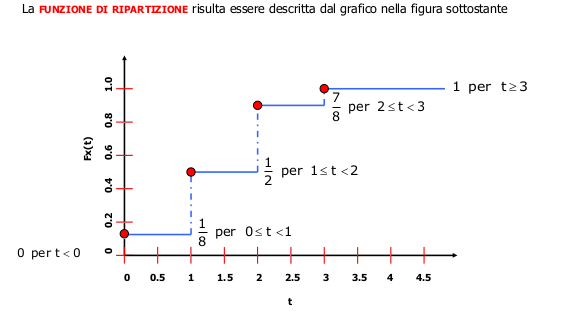
\includegraphics[scale=0.8]{img/rip.png}
\end{center}
Avendo definito la funzione di ripartizione, adesso tutte le questioni riguardanti la variabile casuale $X$
possono trovare una soluzione attraverso di essa, infatti supponiamo di calcolare $P(\{a < X \leq b\})$
con l'evento ${X \leq b}$ esprimibile come l'unione dei due eventi indipendenti ${X \leq a}$ e ${a < X \leq b}$ da cui si ricava,
usando il terzo assioma della probabilità la seguente formula:
\[ \begin{split}
        P(\{X \leq b\}) & = P(\{X \leq a\}) + P(\{a < X \leq b\}) \ \text{da cui si ricava} \\
        P(\{a < X \leq b\}) & = F(b) - F(a) \\
    \end{split} \]
Questa formula ci permette di determinare la probabilità che una variabile casuale possa assumere valori in intervalli reali
e ciò ha un notevole utilizzo in statistica e nella probabilità.

In genere la funzione di ripartizione non è nota, altrimenti tutti gli eventi della nostra vita sarebbero facilmente analizzabili
senza nessuna incertezza, per cui l'obiettivo della statistica è di determinarla o determinare le grandezza ad essa associate
mentre la probabilità e le sue applicazioni assumono che sia sempre nota.
Si dimostra che sono delle funzioni di ripartizione tutte e sole le funzioni del tipo:
\[F:\mathbb{R}\to[0,1]\]
\newpage
che godono simultaneamente delle seguenti proprietà:
\begin{itemize}
\item $F$ è monotona crescente
\item \[\lim_{t\to+\infty} F(t)=1\]
\item \[\lim_{t\to-\infty} F(t)=0\]
\item \[\lim_{t\to t_0^+} F(t)=F(t_0),\,\,\forall t_0\in\mathbb{R}\]
     fnsfgsgsjgjfskshfkj   
\end{itemize}
Le variabili aleatorie si distinguono in due categorie in base alla proprietà di continuità delle corrispondenti funzioni di ripartizione
\subsubsection{Variabile Aleatoria Discreta}
Una variabile aleatoria è detta \textbf{variabile aleatoria discreta} nel caso in cui
l'insieme dei valori $S$ che essa può assumere (supporto) è finito (ovvero costituito
da un numero finito di elementi) o costituito da una infinità di valori discreti. Ad ogni variabile aleatoria discreta si associa, oltre alla funzione di ripartizione, una funzione che fornisce delle valutazioni sulla probabilità che essa assuma specifici valori.\\
Sia $S$ il supporto della variabile aleatoria $X$. Si dice \textbf{distribuzione discreta di probabilità} la funzione:
\[p_X:\mathbb{R}\to[0,1]\]
coì definita:
\[
\begin{cases}
p(X=t)\,\,\,\,  \forall t\in S\\
0\,\,\,\,  altrimenti
\end{cases}
\]
Una funzione $p_X$ definita su un insieme finito $S$ è una distribuzione di probabilità se e solo se sono soddisfatte simultaneamente le seguenti proprietà:
\begin{itemize}
\item \[p_X(t)\geq 0\,\,\,\, t\in \mathbb{R}\]
\item \[\sum_{s\in S} p_X(s)=1\]

\newpage
questa proprietà deriva dalle due precedentemente introdotte:
\begin{itemize}
\item $P(\Omega)=1$
\item data la famiglia $\{A_i,i\in I\subseteq N\}$ 
di eventi incompatibili vale:
\[P(\bigcup_{i\in I} A_i)=\sum_{i\in I} P(A_i)\]
\end{itemize}
\end{itemize}
Tra le funzioni di ripartizione delle variabili discrete e le distribuzioni discrete di
probabilità esiste una corrispondenza biunivoca, nel senso che le une identificano
univocamente le altre. Si ha infatti che:
\begin{itemize}
\item \[F_X(t)=\sum_{s\in S:s\subseteq t} p_X(s)\,\,\, \forall t\in \mathbb{R}\]
\item \[p_X(s)=F_X(s)-\lim_{t\to s^{-}} F_X(t)\,\,\, \forall s\in S\]
\end{itemize}
Dalla prima di tali relazioni se ne deduce che le funzioni di ripartizione delle variabili
aleatorie discrete presentano dei \textit{salti} in corrispondenza dei valori \textit{s} mentre
sono costanti per gli altri valori: per tale ragione vengono dette \textit{funzioni a gradino}.
\subsubsection{Variabile Aleatoria Continua}
Una variabile aleatoria è detta continua nel caso in cui la corrispondente funzione di ripartizione $F_X$ sia continua. In particolare è detta \textbf{assolutamente continua} se esiste una funzione:
\[f_X:\mathbb{R}\to R_+\]
tale che:
\[F_X(t)=\int_{-\infty}^t f_X(u)du\,\,\,\forall t\in \mathbb{R}\]
Una tale funzione quando esista viene detta \textbf{densità di probabilità }di $X$.\\
È detto poi \textbf{supporto} della variabile $X$ l'insieme:
\[S=\{t\in\mathbb{R}:f_X(t)\neq 0\}\]
Si osservi che se la densità di probabilità di una variabile casuale esiste allora la
funzione di ripartizione è una sua primitiva.
Per semplicità supporremo nel seguito che le variabili aleatorie assolutamente
continue abbiano funzione di ripartizione derivabile e che la funzione di densità di
probabilità sia la derivata della funzione di ripartizione.\\
Come per le distribuzioni discrete di probabilità anche le funzioni di densità di
probabilità per essere tali devono soddisfare le seguenti due proprietà:
\begin{enumerate}
\item \[f_X(t)\geq 0\,\,\, \forall t\in \mathbb{R}\]
\item \[\int_{-\infty}^{+\infty}f_X(t)dt=1\]
\end{enumerate}
La probabilità che una variabile aleatoria continua (o
assolutamente continua) assuma un ben determinato valore è sempre nulla. Infatti, se $X$ è una variabile aleatoria continua allora $\forall t_0\in \mathbb{R}$ vale:
\[P(X=t_0)=P(X\leq t_0)-\lim_{t\to t_0^-}P(X\leq t)=F_X(t_0)-\lim_{t\to t_0^-} F_X(t)=F_X(t_0)-F_X(t_0)=0\]
\begin{center}
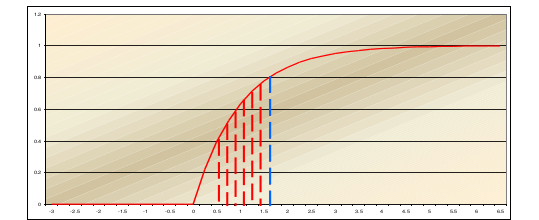
\includegraphics[scale=0.6]{img/con.png}
\end{center}
Pertanto quando si pensa a variabili aleatorie continue, non ha mai senso domandarsi, quale sia la probabilità che esse assumano valori esatti. Al contrario ha senso domandarsi quale sia la probabilità che tali variabili assumano
valori in specifici intervalli dell'asse reale.\\
Per calcolare la probabilità che una variabile casuale continua $X$ assuma un valore in un intervallo $(a,b]\subseteq \mathbb{R}$ è possibile far ricorso alla seguente formula:
\[P(X\in(a,b])=\int_a^b f_X(u)du\,\,\, \forall t\in\mathbb{R}\]
quindi:
\[P(X\in(a,b])=F_X(b)-F_X(a)=\int_{-\infty}^b f_X(u)du-\int_{-\infty}^a f_X(u)du\]
valutiamo in $b$:
\[F_X(b)=\int_{-\infty}^b f_X(u)du=P(X\leq b)\]
che è quindi l'area sottesa alla curva della funzione fino al punto $b$ sull'asse delle $x$.\\
Valutiamo anche in $a$:
\[F_X(a)=\int_{-\infty}^a f_X(u)du=P(X\leq a)\]
che è quindi l'area sottesa alla curva della funzione fino al punto $a$ sull'asse delle $x$.\\
quindi:
\[P(X\in(a,b])=F_X(b)-F_X(a)\]
è l'area sottesa alla curva della funzione fino dal punto $a$ al punto $b$ sull'asse delle $x$.\\
In pratica la probabilità che sia soddisfatto l'evento $X\in(a,b]$ corrisponde all'area sottesa dalla densità $f_X$ nell'intervallo $(a,b]$:
\begin{center}

\psscalebox{1.0 1.0} % Change this value to rescale the drawing.
{
\begin{pspicture}(0,-2.375)(8.38,2.375)
\psbezier[linecolor=black, linewidth=0.04](5.9990716,0.4275487)(5.9981446,1.2275481)(1.6000015,-0.37754923)(1.6009284,-1.1775487080233007)
\psline[linecolor=black, linewidth=0.04, arrowsize=0.05291667cm 2.0,arrowlength=1.4,arrowinset=0.0]{->}(0.8,-2.375)(0.8,2.425)
\psline[linecolor=black, linewidth=0.04, arrowsize=0.05291667cm 2.0,arrowlength=1.4,arrowinset=0.0]{->}(0.4,-1.975)(7.2,-1.975)
\psline[linecolor=black, linewidth=0.04, linestyle=dashed, dash=0.17638889cm 0.10583334cm](1.6,-1.175)(1.6,-1.975)
\psline[linecolor=black, linewidth=0.04, linestyle=dashed, dash=0.17638889cm 0.10583334cm](6.0,0.425)(6.0,-1.975)
\rput[bl](1.6,-2.375){$a$}
\rput[bl](5.6,-2.375){$b$}
\rput[bl](7.2,-2.375){$X$}
\rput[bl](-0.1,2.025){$f_X()$}
\rput[bl](6.4,-0.775){$P(X\in(a,b])$}
\psline[linecolor=black, linewidth=0.04, linestyle=dotted, dotsep=0.10583334cm](5.6,0.425)(2.0,-1.175)
\psline[linecolor=black, linewidth=0.04, linestyle=dotted, dotsep=0.10583334cm](5.6,0.025)(2.0,-1.575)
\psline[linecolor=black, linewidth=0.04, linestyle=dotted, dotsep=0.10583334cm](5.6,-0.375)(2.0,-1.975)
\psline[linecolor=black, linewidth=0.04, linestyle=dotted, dotsep=0.10583334cm](5.6,-0.775)(2.8,-1.975)
\psline[linecolor=black, linewidth=0.04, linestyle=dotted, dotsep=0.10583334cm](5.6,-1.175)(3.6,-1.975)
\psline[linecolor=black, linewidth=0.04, linestyle=dotted, dotsep=0.10583334cm](5.6,-1.575)(4.8,-1.975)
\end{pspicture}
}

\end{center}
quindi:
\[[P(X\in(a,b])=\int_a^bf_X(u)du\,\,\,\forall a,b\in\mathbb{R},\,\,\,a<b\]
inoltre essendo $P(X=a)=0$ si ha:
\[[P(X\in(a,b])=p(X\in[a,b])\,\,\,\forall a,b\in\mathbb{R},\,\,\,a<b\]

Si è visto che per definizione:
\[F_X(t)=\int_{-\infty}^tf_X(u)du\,\,\,\forall t\in\mathbb{R}\]
Ovvero che la funzione di ripartizione è la funzione integrale della funzione di densità di probabilità. Quindi, data la funzione di ripartizione, si ottiene la funzione di densità di probabilità tramite derivazione:
\[\frac{d}{dt}F_X(t)=f_X(t)\]
\subsection{Variabili Aleatorie Multidimensionali}
In molti casi è lecito considerare situazioni (esperimenti) il cui esito è rappresentato, anziché da un valore numerico, da una coppia o da una n-pla di valori, in tal caso si parla di \textit{variabili aleatorie multidimensionali}. Anche qui le variabili sono definite da uno spazio campione $\Omega$ a $\mathbb{R}^n$ con $n$ dimensione della variabile. È comodo pensare a queste variabili aleatorie come a risultati esprimibili da n-ple di valori numerici. Si considerano quindi funzioni che esprimano le valutazioni probabilistiche sui valori assumibili dalle variabili.\\
Consideriamo quindi le \textbf{variabili aleatorie bidimensionali assolutamente continue}, anche se ovviamente si può estendere a $n$ variabili anche non continue. \\
Sia quindi una variabile aleatoria così definita:
\[(X:Y):\Omega\to \mathbb{R}^2\]
con $\Omega$ che è uno spazio campione al quale è associata una probabilità $P$ definita sui sottoinsiemi di $\Omega$.\\
Si definisce la \textbf{funzione di ripartizione congiunta} la funzione bidimensionale:
\[F_{X,Y}(t,s):\mathbb{R}^2\to[0,1]\subseteq \mathbb{R}\]
definita come:
\[F_{X,Y}=P(\{X\leq t\}\cap\{Y\leq s\}\,\,\,\forall (t,s)\in \mathbb{R}\]
inoltre se la variabile $(X,Y)$ è assolutamente continua esiste la \textbf{funzione dei densità congiunta}:
\[f_{X,Y}:\mathbb{R}^2\to \mathbb{R}_+\]
tale che:
\[F_{X,Y}(t,s)=\inf_{-\infty}^t\inf_{-\infty}^s f_{X,Y}(u,v)du\,dv\,\,\,\forall (t,s)\in\mathbb{R}^2\]
conoscendo una delle due funzioni sopra è possibile determinare la probabilità che la coppia $(X,Y)$ assuma
valori in un qualsiasi sottoinsieme rettangolare:
\[(a_1,b_1]\times(a_2,b_2]\in\mathbb{R}^2\]
infatti:
\[P((X,Y)\in (a_1,b_1]\times(a_2,b_2])=F_{X,Y}(b_1,b_2)-F_{X,Y}(a_1,b_2)-F_{X,Y}(b_1,a_2)+F_{X,Y}(a_1,a_2)\]
\[=\int_{a_1}^{b_1}\int_{a_2}^{b_2} f_{X,Y}(u,v) du\,dv\,\,\, \forall (a_1,b_1]\times(a_2,b_2]\in\mathbb{R}^2\]
\begin{center}
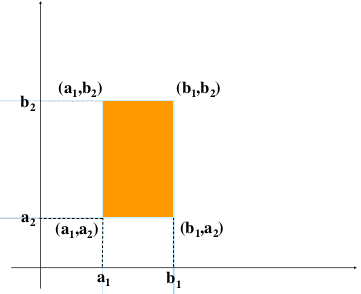
\includegraphics[scale=0.7]{img/mul.png}
\end{center}
In molti casi, benché ci si trovi di fronte a situazioni i cui esiti sono di tipo multidimensionale, capita di essere interessati ai valori che possono essere assunti
solamente da una delle variabili. Si introducono quindi le \textbf{funzioni marginali}.\\
Data una variabile aleatoria bidimensionale $(X,Y)$ assolutamente continua, avente funzione di ripartizione congiunta $F_{X.Y}$ e funzione di densità disgiunta $f_{X,Y}$
è detta \textbf{funzione di ripartizione marginale di X}:
\[F_X(t)=P(\{X\leq t)\}\cap\{Y\leq +\infty\})=F_{X,Y}(t,+\infty)\]
ed p detta \textbf{funzione di densità marginale di X}:
\[f_X(t)=\int_{-\infty}^{+\infty}f_{X.Y}(t,s)\,ds\]
Data una variabile bidimensionale $(X;Y)$ diciamo che le due variabili considerate singolarmente sono \textbf{stocasticamente indipendenti} sse $\forall (t,s)\in\mathbb{R}^2$ vale:
\[F_{X,Y}(t,s)=F_X(t)\cdot F_Y(s)\]
che è equivalente a:
\[P(\{X\in A)\}\cap\{Y\in B\})=(X\in A)\cdot P(Y\in B)\,\,\,\forall A,B\\subseteq \mathbb{R}\]
che equivale, se la coppia di variabili è assolutamente continua, a:
\[f_{X,Y}(t,s)=f_X(t)\cdot f_Y(s)\,\,\,\forall (t,s)\in \mathbb{R}^2\]
\section{Indici}
\subsection{Indici di tendenza centrale}
Sono grandezze numeriche associate alle variabili aleatorie in grado di sintetizzare, con un solo valore, le principali caratteristiche delle loro distribuzioni. Risultano strettamente legati agli indici introdotti nella prima parte in relazione alla statistica descrittiva. Il più importante degli indici di tendenza centrale è detto \textbf{valore atteso} corrispondente alla media matematica dei dati statistici.\\
Data una variabile aleatoria unidimensionale $X$ avente supporto $S\subseteq \mathbb{R}$ è detto valore atteso di $X$ la quantità:
\[E[X]\begin{cases}
\sum_{s\in S}\,\, s\cdot p_X(s)\mbox{ se X è discreta}\\
\\
\int_{-\infty}^{+\infty}\,\, u\cdot f_X(u)\,du\mbox{ se X è assolutamente continua}\\
\end{cases}\]
e notiamo l'analogia con la formula del valor medio per una serie di dati:
\[\overline{x})\sum_{j=1}^N s_jp_j=s_1p_1+\cdots +s_Np_N\]
In effetti il valore atteso, così come la media di una serie di dati, va pensato come una \textit{media pesata} dei valori assumibili dalla variabile, e fornisce un'indicazione di
massima del posizionamento della variabile lungo l'asse dei numeri reali. Il valore atteso gode delle seguenti tre proprietà:
\begin{enumerate}
\item $\forall a\in\mathbb{R}$, se $X=a$ con probabilità uguale ad 1 allora $E[X]=a$
\item $E[a\cdot X+b]=a\cdot E[X]+b$ per ogni variabile $X$ e per ogni $a,b \in\mathbb{R}$
\item data una funzione $y=g(X)$ della variabile aleatoria $X$ si ha che il valore atteso è:
\[E(g(X)]=\int_{-\infty}^{+\infty}g(u)f_X(u)\,du\]
\end{enumerate}
\textbf{Niente assicura che il valore atteso di una variabile esista}, infatti è definito mediante un integrale improprio e si ha quando ho la sommatoria o l'integrale non convergono\\
Il valore atteso è in realtà un caso particolare di momento centrale, $\forall r = 1,2, \cdots$,è detto \textbf{momento centrale di \textit{X} di ordine \textit{r}} la quantità:
\[E[X^r]\begin{cases}
\sum_{s\in S}\,\, s^r\cdot p_X(s)\mbox{ se X è discreta}\\
\\
\int_{-\infty}^{+\infty}\,\, u^r\cdot f_X(u)\,du\mbox{ se X è assolutamente continua}\\
\end{cases}\]
Un altro indice di tendenza centrale è la \textbf{moda} di una variabile aleatoria $X$, indicata con $\widetilde{X}\in\mathbb{R}$, corrispondente al valore per cui è massima la distribuzione discreta di probabilità (se $X$ è discreta) oppure la funzione di densità (se $X$ è assolutamente continua). Non è detto che un tale valore sia unico, se lo è diremo che la distribuzione di X è \textit{unimodale}, in caso contrario si parlerà di distribuzione \textit{multimodale}. Può capitare in alcuni casi che la distribuzione discreta di probabilità o la funzione
di densità presentino diversi punti di massimo locale.
Sebbene ciò non sarebbe formalmente corretto, tutti questi punti di massimo locale vengono solitamente considerati come punti modali e pertanto anche in questo caso si parla di distribuzione multimodale.\\
Un terzo indice di tendenza centrale è la \textbf{mediana}  di una variabile aleatoria $X$, indicata con $\hat{X}\in\mathbb{R}$, che soddisfa la diseguaglianza:
\[lim_{t\to \hat{X}^-} F_X(t)\leq \frac{1}{2}\leq F_X(\hat{X})\]
Nel caso in cui la funzione di ripartizione della variabile sia continua ed invertibile allora:
\[\hat{X}=F_X^{-1}(\frac{1}{2})\]
Nel caso di variabili discrete invece la mediana è il valore dell'ascissa in cui la funzione di ripartizione passa da un valore minore di $\frac{1}{2}$ ad uno superiore. Più semplicemente è possibile pensare alla mediana come a quel valore per cui sia la probabilità che X assuma valori più piccoli che la probabilità che X assuma valori più grandi sono pari a $\frac{1}{2}$. La mediana può non essere unica e ciò si verifica quando esistano più valori $t$ per i quali risulti:
\[F_X(t)=\frac{1}{2}\]
\begin{center}
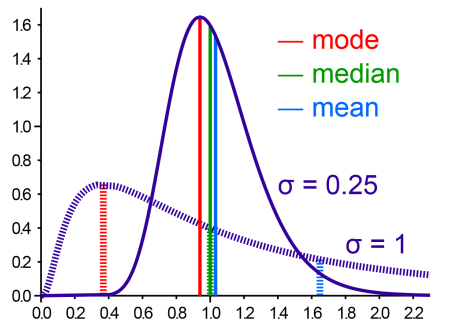
\includegraphics[scale=0.7]{img/mmm.png}
\end{center}
Unitamente alla mediana è possibile considerare altri indici definiti in maniera simile e che dividono la retta dei reali in due intervalli di probabilità assegnata e che sono detti \textbf{quantili}. Dato un valore $P\in[0,1]\subseteq\mathbb{R}$ è detto \textbf{quantile p-esimo della variabile aleatoria X} il valore:
\[x_p in\mathbb{R}:\lim_{t\to x_p^{-}}F_X(t)\leq p\leq F_X(x_p)\]
Nel caso in cui la funzione di ripartizione sia continua ed invertibile allora:
\[x_p=F_X^{-1}(p)\]
per cui pensiamo a $x_p$ come ad un valore per cui risulta:
\[P(X\leq x_p)=p\mbox{ e } P(X>x_p)=1-p\]
\begin{center}
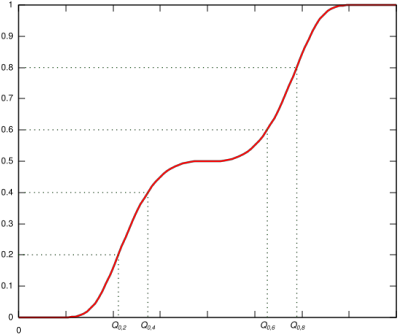
\includegraphics[scale=0.5]{img/qua.png}
\end{center}
\subsection{Indici di variabilità}
Come visto in precedenza oltre agli indici di tendenza centrale è conveniente anche considerare indici che forniscano un'idea del grado di dispersione
dei valori assumibili da una variabile aleatoria.
Questi vengono detti \textbf{indici di variabilità}. Il più famoso tra tutti è la \textbf{varianza} di una variabile aleatoria $X$ definita come:
\[V[X]\begin{cases}
\sum_{s\in S}\,\, (s-E[X])^2\cdot p_X(s)\mbox{ se X è discreta}\\
\\
\int_{-\infty}^{+\infty}\,\, (u-E[X])^2\cdot f_X(u)\,du\mbox{ se X è assolutamente continua}\\
\end{cases}\]
Così come il valore atteso anche la varianza talvolta può non esistere, quando la
sommatoria o l'integrale divergono.
Così come il valore atteso di una variabile aleatoria$ X$ viene spesso indicato con $\mu_X$ si ha che la varianza viene indicata con $\sigma_X^2$.\\
La radice della varianza è un altro indice importante ed è detto \textbf{deviazione standard}, ha il vantaggio rispetto alla varianza di avere la stessa unità di misura del valore atteso:
\[\sigma_X=\sqrt{s_X^2}\]
La varianza ha le seguenti proprietà:
\begin{enumerate}
\item $\forall a\in\mathbb{R}$, se $X=a$ con probabilità uguale ad 1 allora $V[X]=0$
\item $V[a\cdot X+b]=a^2\cdot V[X]+b$ per ogni variabile $X$ e per ogni $a,b \in\mathbb{R}$
\item $V[X]=E[X^2]-(E[X])^2\,\,\forall X$ variabile aleatoria
\end{enumerate}
\subsection{Indici multidimensionali}
Anche per le variabili multidimensionali ed in particolare per quelle bidimensionali esistono indici di tendenza centrale e variabilità.\\
Sia $(X,Y)$ una variabile aleatoria bidimensionale discreta o continua. Sono detti \textbf{valori attesi marginali} e \textbf{varianza marginali }le quantità:
\[E[X]\,\,E[Y]\,\,V[Y]\,\,V[Y]\]
ottenute considerando le distribuzioni marginali di $X$ ed $Y $ ed integrando (o sommando) in accordo ai sistemi visti sopra.\\
Si hanno le seguenti relazioni:
\begin{itemize}
\item $E[a\cdot X +b \cdot Y]=a\cdot E[X] + b\cdot E[Y]\,\,\forall \mbox{ coppia }X,Y \mbox{ e }\forall a,b\in\mathbb{R}$
\item $E[X \cdot Y]= E[X]\cdot E[Y]\,\,\forall \mbox{ coppia }X,Y \mbox{ stocasticamente indipendenti}$
\item $V[X + Y]= V[X]+ V[Y]\,\,\forall \mbox{ coppia }X,Y \mbox{ stocasticamente indipendenti}$
\end{itemize}
Oltre ai valori attesi ed alle varianze marginali, un altro indice è estremamente importante, si tratta della \textbf{covarianza} definita come:
\[Coc[X,Y]=E[(X-E[X])\cdot(Y-e[X])]=\iint_{\mathbb{R}^2} (t-E[X])\cdot (s-E[Y])\cdot f_{X,Y}(t,s)\,dt\,ds\]
\[=\iint_{\mathbb{R}^2} t \cdot s\cdot f_{x,y}(t,s)\,dt\,ds-\int_{\mathbb{R}}t\cdot f_X(t)dt\cdot \int_{\mathbb{R}}s\cdot f_Y(s)dt\]
La covarianza è un indice della correlazione che sussiste tra due variabili ovvero del loro grado di dipendenza reciproca.
Tanto più essa è grande tanto più forte è il legame di dipendenza tra le variabili. Si noti ad esempio che se le variabili X ed Y sono stocasticamente indipendenti si ottiene (a partire dalla seconda relazione sopra nominata per $E[X\cdot Y]$) che:
\[Cov[X,Y]=E[X\cdot Y]-E[X]\cdot E[Y]=E[X]\cdot E[Y]-E[X]\cdot E[Y]=0\]
Due variabili aleatorie aventi covarianza nulla vengono dette \textbf{incorrelate}. Occorre però sottolineare che la nozione di incorrelazione è più debole di quella di
indipendenza. Infatti, è possibile mostrare che seppur esistano coppie di variabili incorrelate esse
non sono indipendenti.\\
Un ultimo indice è quello detto \textbf{coefficiente di correlazione di Pearson}, strettamente legato alla covarianza ed utilizzato per esprimere più chiaramente il grado di dipendenza tra due variabili:
\[p_{XY}=\frac{Cov[X,Y]}{\sqrt{V[X]\cdot V[Y]}}=\frac{Cov[X,Y]}{\sigma_x\cdot \sigma_y}\]
questo indice ha le seguenti proprietà:
\begin{enumerate}
\item $p_{XY}=0$ se $X$ e $Y$ sono incorrelate
\item $|p_{XY}|=1$ se vale la relazione $Y=a\cdot X+b\,\,\,\forall a,b\in \mathbb{R}$
\end{enumerate}
Ovvero se vale $+1$ allora $a>0$ e se vale $-1$ si ha che $a<0$
\newpage
\section{Esercizi}
\begin{esercizio}
2 carte con reintroduzione si estraggono da un mazzo da 52.
\begin{enumerate}

\item P che prima sia di picche seconda di quadri
\item P di due figure dello stesso seme
\item se la prima è > 4 calcolo P che la seconda sia 10

\end{enumerate}
risposte:
\begin{enumerate}

\item P1 prima carta picche e Q2 seconda carta quadri. Sono eventi indipendenti per la reintroduzione
\[P(P1\cap Q2)=P(P1)\cdot P(Q2)=\frac{13}{52}\cdot \frac{13}{52}=\left(\frac{13}{52}\right)^2\]
\item A carta di seme X e B carta di seme X, si ricorda reintroduzione
\[P(A\cap B)=P(A)\cdot P(B|A)=\frac{12}{52}\cdot \frac{3}{52}= \frac{9}{876}\]
\item C carta > 4 e D carta = 10, la carta è sempre la stessa
\[P(D|C)=\frac{P(D\cap C)}{P(C)}=\frac{P(D)}{P(C)}=\frac{1}{9}\]
\end{enumerate}
\end{esercizio}
\begin{esercizio}
Gli abitanti di abc raggiungono xyz col treno con con la macchina. Il 90\% arriva in ritardo, il 40\% di questi usa il treno. Il 20\% di quelli che non arriva in ritardo usano la macchina.
\begin{enumerate}
\item probabilità che un abitante usi il treno
\item se usa il treno percentuali di ritardo o meno
\end{enumerate}
risposte
\begin{enumerate}
\item R = 0.9 persona in ritardo, $\overline{R}=0.1$ non in ritardo, T usa treno e M usa macchina\\
\[P(T)=P(R)\cdot P(T|R)+P(\overline{R})\cdot P(T|\overline{R})=0.9*0.4+0.1*0.8=0.44\]
\item \[P(R|T)=\frac{P(R\cap T)}{P(T)}=\frac{P(T|R)\cot P(R)}{P(T)}=\frac{0.9*0.4}{0.44}=0.8182\]
quindi per la macchina è $1-0.8182=0.1818$
\end{enumerate}
\end{esercizio}
\begin{esercizio}
Un urna contiene una pallina rossa e una bianca, ne estraggo una e la rimetto dentro con un'altra dello stesso colore. All'i-sima estrazione se ne estrae una rossa (Ri) e all'i-esima estrazione una bianca(Bi)
\begin{enumerate}
\item P(R2) alla seconda estrazione una rossa e P(R3) alla terza estrazione una rossa
\item se la seconda è rossa la prima era più probabile bianca o rossa?
\item P di avere prima rossa e seconda bianca
\end{enumerate}
risposta:
\begin{enumerate}
\item \[P(R2)=P(R1\cap R2)+P(B1\cap R2)=\]
\[P(R1\cap R2)=P(R1)\cdot P(R2|R1)= \frac{1}{2}\cdot \frac{2}{3}=\frac{1}{3}\]
\[P(B1\cap R2)=P(B1)\cdot P(R2|B1)=\frac{1}{2}\cdot \frac{1}{3}=\frac{1}{6}\]
\[P(R2)=\frac{1}{2}\]
\[P(R3)=P(R1\cap R2\cap R3)+P(R1\cap B2\cap R3)+P(B1\cap R2\cap R3)+P(B1\cap B2\cap R3)\]
\[P(R1\cap R2\cap R3)=P(R1)\cdot P(R2|R1)\cdot P(R3|R1\cap R2)=\frac{1}{2}\cdot \frac{2}{3}\cdot \frac{3}{4}=\frac{1}{4}\]
\[P(R1\cap B2\cap R3)=P(R1)\cdot P(B2|R1)\cdot P(R3|R1\cap B2)=\frac{1}{2}\cdot \frac{1}{3}\cdot \frac{1}{2}=\frac{1}{12}\]
\[P(B1\cap R2\cap R3)=P(B1)\cdot P(R2|R1)\cdot P(R3|R1\cap R2)=\frac{1}{2}\cdot \frac{1}{3}\cdot \frac{1}{2}=\frac{1}{12}\]
\[P(B1\cap B2\cap R3)=P(B1)\cdot P(B2|R1)\cdot P(R3|R1\cap B2)=\frac{1}{2}\cdot \frac{2}{3}\cdot \frac{1}{4}=\frac{1}{12}\]
\[P(R3)=\frac{1}{4}+\frac{1}{12}+\frac{1}{12}+\frac{1}{12}=\frac{1}{2}\]
\item \[P(R1|R2)=\frac{P(R1\cap R2}{P(R2)}=\frac{P(R1)\cdot P(R2|R1}{P(R2)}=\frac{\frac{1}{2}\cdot \frac{2}{3}}{\frac{1}{2}}=\frac{2}{3}\]
\[P(B1|R2)=\frac{P(B1\cap R2}{P(R2)}=\frac{P(B1)\cdot P(R2|B1}{P(R2)}=\frac{\frac{1}{2}\cdot \frac{1}{3}}{\frac{1}{2}}=\frac{1}{3}\]
\item \[P(R1\cap B2)=P(R1)\cdot P(B2|R1)=\frac{1}{2}\cdot \frac{1}{3}=\frac{1}{6}\]
\end{enumerate}
\end{esercizio}
\chapter{Distribuzioni Notevoli}
Si parla di \textbf{distribuzione} di una variabile indentendo indifferentemente la sua ripartizione o la sua densità (o distribuzione di
probabilità). Nel seguito presenteremo dapprima le distribuzioni discrete e successivamente le distribuzioni assolutamente continue. Con 
\[X\sim F\]
si indica che la variabile X è distribuita secondo F.\\
Una variabile aleatoria X è detta distribuita secondo una Bernoulliana di parametro $p\in[0,1]$
\[X\sim B(p)\]
se  essa può assumere solo i valori 1 e 0 rispettivamente con probabilità $p$ e $(1-p)$:
\[p_X(t)=\begin{cases}
1-p\mbox{ se } t=0\\
p \mbox{ se } t=1\\
0 \mbox{ altrimenti} 
\end{cases}\]
\[F_X(t)=\begin{cases}
0\mbox{ se } t=0\\
1-p \mbox{ se } 0\leq t<1\\
1 \mbox{ se } t\geq 1 
\end{cases}\]
L’importanza di questa semplice distribuzione è ovvia, sono variabili di Bernoulli tutte quelle che individuano il verificarsi di uno specifico evento e che valgono 1 se questo si verifica e 0 altrimenti. Determino quindi media e mediana di una bernoulliana:
\[E[X]=0\cdot (1-p)+1\cdot p= p\]
\[V[X]=[0^2\cdot(1-p)+1^2\cdot p]=(1-p)\cdot p\]
Siano $X_1,\cdots, X_n$ n variabili Bernoulliane di identico parametro p e stocasticamente indipendenti tra loro. Sia $X=\sum X_i$ Una tale variabile è detta distribuita secondo una Binomiale con parametri $n$ e $p$:
\[X\sim Bin(n,p)\]
Una tale variabile può assumere qualsiasi valore intero $k$ compreso tra 0 ed $n$ in accordo alla seguente probabilità:
\[P(X=k)=\binom{n}{k}\cdot p^k\cdot (1-p)^{n-k}\]
infatti $p^k\cdot (1-p)^{n-k}$ fornisce la probabilità che $k$ delle n variabili Xi assumano il valore 1 e che le restanti
$(n-k)$ assumano valore 0. Inoltre si ricorda che;
\[\binom{n}{k}=\frac{n!}{(n-k)!\cdot k!}\]
esprime il numero di combinazioni possibili per cui $k$ variabili valgono 1 e $(n-k)$ valgono 0.\\
la \textit{distribuzione di probabilità} e la \textit{funzione di ripartizione} risultano essere quindi:
\[p_X(t)=\begin{cases}
\binom{n}{t}p^t(1-p)^{n-t} \mbox{ se } t\in\{0,\cdots, n\}\\
0 \mbox{ altrimenti } 
\end{cases}\]
\[F_X(t)=\sum_{0\leq k\leq n;k\leq t}\binom{n}{k}p^k(1-p)^{n-k},\,\,\forall t\in \R\]
Le variabili $X_i$ sono indipendenti quindi posso calcolare il valore atteso e la varianza di $X$:
\[E[X]=E[X_1+\cdots+X_n]=E[X_1]+\cdots+E[X_n]=n\cdot p\]
\[V[X]=V[X_1+\cdots+X_n]=V[X_1]+\cdots+V[X_n]=n\cdot (1-p)\cdot p\]
La principale applicazione della distribuzione binomiale consiste nella definizione di variabili che "contano" le realizzazioni di eventi quando questi siano da considerarsi indipendenti e con identica probabilità di verificarsi.\\
\begin{center}
	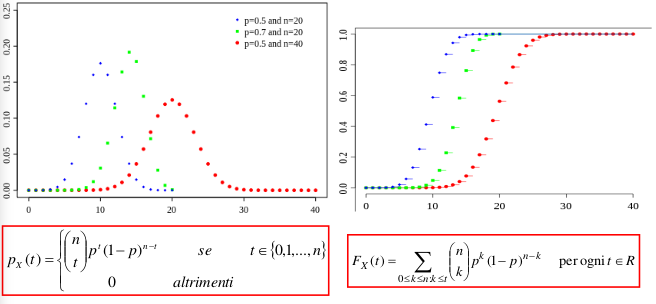
\includegraphics[scale=0.7]{img/dis5.png}
\end{center}
La distribuzione di Poisson può essere vista come un caso particolare della
distribuzione Binomiale che si ottiene quando il numero di variabili $X_i$ che compaiono in:
\[X=\sum X_i\]
tende ad infinito mentre il valore del parametro $p$ tende a zero in modo tale che il prodotto $n\cdot p$ resti costante. Assumiamo:
\[\lambda = n\cdot p\]
quindi $X$ è distribuita secondo una Poisson con parametro $\lambda\in\R_+$:
\[X\sim Poi(\lambda)\]
Ovviamente una variabile così definita mappa in $\R$. Qualcolo la rpobabilità associata:
\[P(X=k)=\lim_{n\to+\infty} \binom{n}{k}\cdot p^k\cdot (1-p)^{n-k}=\frac{\lambda^k}{k!}e^{-\lambda},\,\,\forall k\in\mathbb{N}\]
la \textit{distribuzione di probabilità} e la \textit{funzione di ripartizione} risultano essere quindi:
\[p_X(t)=\begin{cases}
\frac{\lambda^k}{k!}e^{-\lambda} \mbox{ se } t\in\{0,\cdots, n\}\\
0 \mbox{ altrimenti}
\end{cases}\]
\[F_X(t)=\sum_{k\in\mathbb{N}:k\leq t}\frac{\lambda^k}{k!}e^{-\lambda},\,\,\forall t\in\R \]
valore atteso e varianza le ricavo da quelli delle bernoulliane con $\lambda=n\cdot p$:
\[E[X]=n\cdot p=\lambda\]
\[V[X]=n\cdot (1-p)\cdot p=n\cdot p-n\cdot p^2= \lambda-\frac{\lambda^2}{n}\]
che con $n\to +\infty$ diventa $V [X]=\lambda$\\
La distribuzione di Poisson viene utilizzata quando si considerino grandi popolazioni di individui in cui ogni individuo ha una probabilità p molto piccola di essere soggetto ad uno specifico evento in esame. Per tale ragione la distribuzione di Poisson viene anche detta degli eventi rari.\\
\begin{center}
	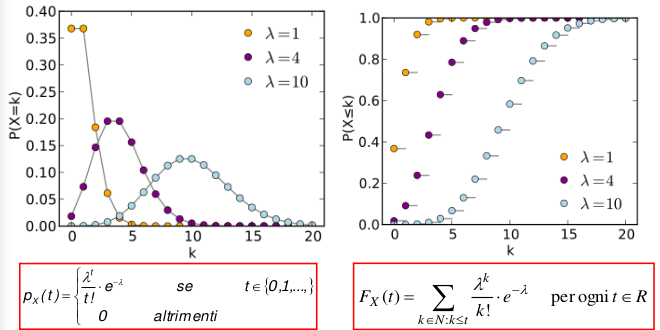
\includegraphics[scale=0.7]{img/dis4.png}
\end{center}

Una variabile aleatoria X è detta distribuita secondo una Geometrica di parametro $p\in[0,1]$:
\[X\sim Geo(p)\]
se può assumere qualsiasi valore intero non negativo k con probabilità:
\[P(X=k)=p\cdot (1-p)^k\]
la \textit{distribuzione di probabilità} e la \textit{funzione di ripartizione} risultano essere quindi:
\[p_X(t)=\begin{cases}
p\cdot (1-p)^t \mbox{ se } t\in\mathbb{N}\\
0 \mbox{ altrimenti}
\end{cases}\]
\[F_X(t)=\sum_{k\in\mathbb{N}:k\leq t}p\cdot(1-p)^k,\,\,\forall t\in\R \]
con valore atteso e varianza:
\[E[X]=\frac{1-p}{p}\]
\[V[X]=\frac{1-p}{p^2}\]
L'importanza di questa distribuzione sta nella \textbf{proprietà di assenza di memoria}:
\[P(X=k+m|X\geq m)=P(X=k)\]
\begin{center}
	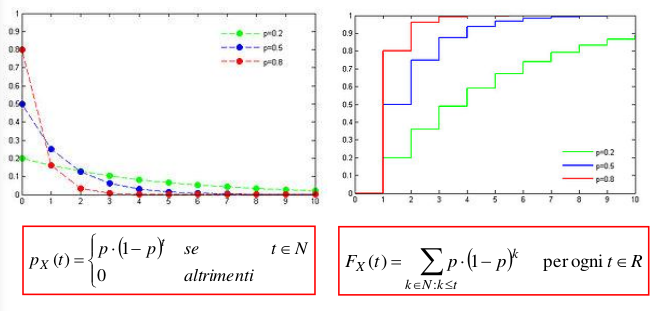
\includegraphics[scale=0.7]{img/dis3.png}
\end{center}
Per comprenderne il significato, supponiamo che X sia il tempo di vita di una macchina soggetta a guasti (possono avvenire solo in corrispondenza di intervalli di tempo unitari), e supponiamo di aver rilevato che per m unità di tempo essa non si sia guastata.\\
La proprietà di assenza di memoria A asserisce che la probabilità che la macchina si guasti all'istante $(k+m)$-esimo, condizionata dall'evento $X\geq m$, è uguale alla probabilità iniziale che essa si guasti all'istante k-esimo. Quindi questa proprietà asserisce che il tempo trascorso
da quando abbiamo iniziato ad esaminare il funzionamento della macchina non influisce sulla distribuzione del tempo restante al verificarsi del guasto.\\
Parliamo ora della \textbf{distribuzione uniforme}. Rappresenta la più semplice distribuzione assolutamente continua e viene adottata
nel caso in cui la variabile considerata possa assumere qualsiasi valore compreso in un dato intervallo con probabilità costante. Si dice che la variabile $X$ è distribuita secondo una uniforme di supporto $[a,b]$:
\[X\sim U[a,b]\]
se essa è assolutamente continua con densità e funzione di ripartizione:
\[f_X(t)=\begin{cases}
\frac{1}{b-a} \mbox{ se } t\in[a,b]\\
0 \mbox{ altrimenti}
\end{cases}\]
\[F_X(t)=\begin{cases}
0 \mbox{ se } t<a\\
\frac{t-a}{b-a} \mbox{ se } t\in[a,b]\\
1 \mbox{ se } t> b
\end{cases}\]
e con semplici integrazioni è possibile ricavare il valore atteso e la varianza:
\[E[X]=\frac{a+b}{2}\]
\[V[X]=\frac{(b-a)^2}{12}\]
Come accennato in precedenza l'interesse in questa distribuzione è giustificato dal
fatto che essa descrive bene situazioni nelle quali le variabili possono assumere valori in intervalli finiti di $\R$ con probabilità uniforme ovvero tale da essere identica per intervalli di medesima ampiezza (purchè contenuti nel supporto della variabile stessa).\\
\begin{center}
	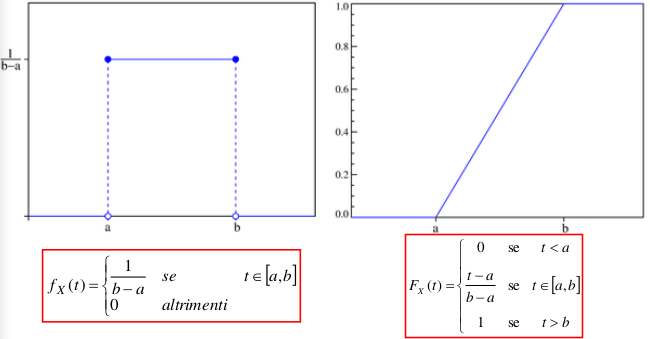
\includegraphics[scale=0.7]{img/dis2.png}
\end{center}

Ovviamente non è certo che i valori assumibili abbiano tutti la stessa probabilità di presentarsi. Per questa ragione sono state introdotte in letteratura diverse generalizzazioni
della distribuzione uniforme. Una di queste è la\textbf{ distribuzione triangolare}, che assegna alla densità di probabilità valori maggiori al centro del supporto e minori in prossimità degli estremi.\\
Formalmente diciamo che la variabile $X$ è
distribuita secondo una Triangolare di supporto $[a,b]$:
\[X\sim T[a,b]\]
se essa è assolutamente continua con \textbf{densità} e \textbf{funzione di ripartizione}:
\[f_X(t)=\begin{cases}
\frac{4(t-a)}{(b-a)^2} \mbox{ se } t\in\left[a,\frac{a+b}{2}\right)\\
\frac{4(b-t)}{(b-a)^2} \mbox{ se } t\in\left[\frac{a+b}{2},b\right]\\
0 \mbox{ altrimenti}
\end{cases}\]
\[F_X(t)=\begin{cases}
0 \mbox{ se } t<a\\
\frac{2(t-a)^2}{(b-a)^2} \mbox{ se } t\in\left[a,\frac{a+b}{2}\right)\\
1-2\frac{(b-t)^2}{(b-a)^2} \mbox{ se } t\in\left[\frac{a+b}{2},b\right]\\
1 \mbox{ se } t>b\\
\end{cases}\]
e integrando si ottengono \textbf{valor medio} e \textbf{varianza}:
\[E[X]=frac{a+b}{2}\]
\[V[X]=\frac{(b-a)^2}{24}\]
\newpage
Passiamo alla \textbf{distribuzione esponenziale}.  Questa distribuzione è particolarmente importante nello studio di quelle variabili che
descrivono i tempi occorrenti al verificarsi di un evento. Formalmente, una variabile aleatoria $X$ è distribuita secondo una Esponenziale di
parametro $\lambda\in\R$:
\[X\sim Exp(\lambda)\]
se essa è assolutamente continua on \textbf{densità} e \textbf{funzione di ripartizione}:
\[f_X(t)=\begin{cases}
\lambda e^{-\lambda t} \mbox{ se } t\geq 0\\
0 \mbox{ altrimenti}
\end{cases}\]
\[F_X(t)=\begin{cases}
1-e^{-\lambda t} \mbox{ se } t\geq 0\\
0 \mbox{ altrimenti}
\end{cases}\]
e integrando si ottengono \textbf{valor medio} e \textbf{varianza}:
\[E[X]=\frac{1}{\lambda}\]
\[V[X]=\frac{1}{\lambda^2}\]
L'importanza della distribuzione esponenziale in numerosi campi applicativi è dovuta al fatto che essa è l’unica distribuzione assolutamente continua che gode della \textbf{proprietà di assenza di memoria}:
\[P(X>s+t|X>s=P(Z>t)\]
\begin{center}
	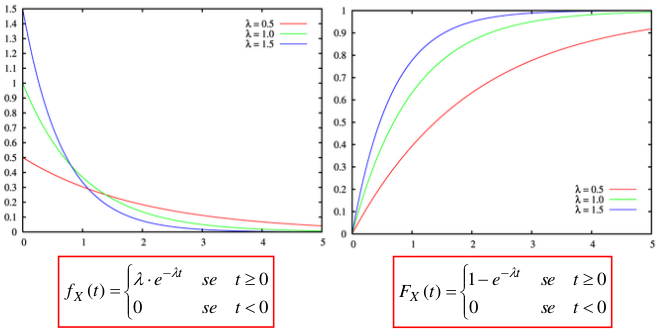
\includegraphics[scale=0.7]{img/dis.png}
\end{center}
\subsection{Distribuzione Normale}
Una variabile aleatoria X è detta \textbf{distribuita secondo una Normale con parametri} $\mu\in\R$ e $\sigma\in\R_+$:
\[X\sim N(\mu,\sigma)\]
se essa è assolutamente continua con densità:
\[f_X(t)=\frac{1}{\sqrt{2\cdot \pi\cdot \sigma^2}}\cdot e^{-\frac{(t-\mu)^2}{2\cdot \sigma^2}}\,\,\,\forall t\in\R\]
Questa distribuzione è fondamentale per il \textbf{teorema centrale del limite}.\\
Integrando si ottengono il valore atteso e la varianza:
\[E[X]=\mu\]
\[V[X]=\sigma^2\]
Inoltre, la variabile aleatoria ha supporto su tutto l'asse reale:
\begin{center}
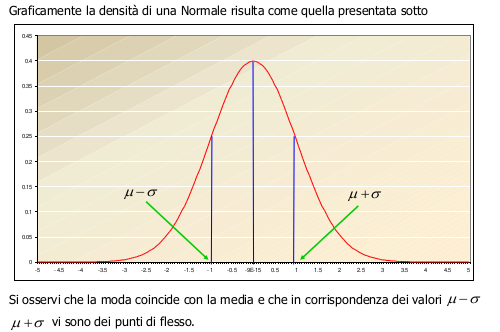
\includegraphics[scale=0.7]{img/norm.png}
\end{center}
\begin{center}
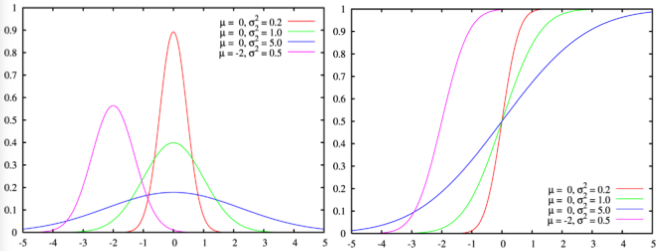
\includegraphics[scale=0.7]{img/nomr2.png}
\end{center}
Non però facile calcolare la P che la variabile casa in un intervallo $[a,b]$:
\[P(X\in[a,b])?\int_a^b \frac{1}{\sqrt{2\cdot \pi\cdot \sigma^2}}\cdot e^{-\frac{(t-\mu)^2}{2\cdot \sigma^2}}\,dt\]
Per questa ragione si ricorre ad opportune tavole che si riferiscono alla distribuzione
normale standard ovvero con parametri $\mu=0$ e $\sigma=1$ e che forniscono i valori di:
\[\int_0^z f_X(t(\,dt\]
per un elevato numero di valori $z\in\R$.\\
Quando si sia interessati a determinare delle probabilità associate ad una generica:
\[X\sim N(\mu,\sigma)\]
ci si riconduce al caso sopra osservando che la variabile:
\[Z=\frac{X-\mu}{\sigma}\]
è distribuita secondo una \textbf{Normale Standard} ovvero si ha che:
\[\mbox{se }X\sim N(\mu,\sigma)\mbox{ allora }Z=\frac{X\mu}{\sigma}\sim N(0,1)\]
quindi ogni variabile $X\sim N(\mu,\sigma)$ può essere ricondotta ad una può essere ricondotta ad
una Normale Standardizzata ovvero ancora per ogni ovvero ancora $\forall [a,b]\subseteq\R$ si avrà:
\[P(X\in[a,b])=P(a\leq X\leq b)=P\left(\frac{a-\mu}{\sigma}\leq \frac{X-\mu}{\sigma}\leq \frac{b-\mu}{\sigma}\right)=P\left(Z\in\left[\frac{a-\mu}{\sigma},\frac{a-\mu}{\sigma}\right]\right)\]
Si ha la \textbf{proprietà di chiusura rispetto alla somma di variabili aleatorie stocasticamente indipendenti:}
\[\mbox{se }X_1\sim N(\mu_1,\sigma_1)\mbox{ e }X_2\sim N(\mu_2,\sigma_2)\]
e se $X_1$ e $X_2$ sono indipendenti allora la viabile $Y=X_1+X_2$ è tale che:
\[Y\sim N(\mu_1+\mu_2,\sqrt{\sigma_1^2+\sigma_2^2})\]
In altri termini la variabile somma di due variabili aleatorie stocasticamente indipendenti con distribuzioni normali è ancora una variabile aleatoria distribuita
secondo una normale i cui parametri sono ricavabili facilmente da quelli delle distribuzioni degli addendi.\\
\begin{shaded}
\subsubsection{La tabella della z}
una volta ottenuto $P\left(Z\in\left[\frac{a-\mu}{\sigma},\frac{a-\mu}{\sigma}\right]\right)$ poniamo per semplicità $\gamma= \frac{a-\mu}{\sigma}$ e $\delta=\frac{a-\mu}{\sigma}$. Per simmetria notiamo che è indifferente valutare $\gamma$ e $\delta$ sia che siano positivi che negativi e per comodità la tabella presenta unicamente valori positivi. Valutemo quindi $|\gamma|$ e $|\delta|$. Sappiamo che $P(Z\in[\gamma,\delta])=P(Z\in[0, |\gamma|])+P(Z\in[0,|\delta|])$. Per calcolare, per esempio, $P(Z\in[0, |\gamma|])$ prendo la cifra intera e la prima cifra decimale e trovo la riga corrispondente nella prima colonna (se $\gamma=1.35$ cercherò $1.3$) e poi cerco scelgo la colonna corrispondente al valore della seconda cifra decimale presente nella prima riga (nel caso di prima cerco nella prima riga il valore $0.05$ e ne scelgo la colonna). L'incrocio fra la riga scelta prima e la colonna scelta dopo mi daranno il valore ricercato. Ecco un esempio con 0.08 e 1.35:
\begin{center}
	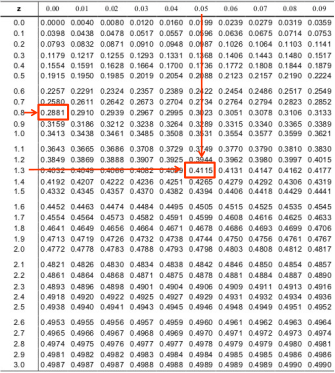
\includegraphics[scale=0.68]{img/z2.png}
\end{center}
\end{shaded}
\begin{shaded}
Regole di calcolo per normali standardizzati da tabelle per integrali:
\begin{itemize}
	\item integrali della forma $\int_{-\infty}^bf(u)\,du$:
	\begin{itemize}
		\item $b>0$, finito:
			\[\int_{-\infty}^b f(u)\, du= \frac{1}{2}+\int_0^b f(u)\, du\]
		\item $b<0$, finito:
			\[\int_{-\infty}^b f(u)\, du= \frac{1}{2}-\int_0^{-b} f(u)\, du\]
	\end{itemize}
	\item integrali della forma $\int_{a}^{+\infty}f(u)\,du$:
		\[\int_{a}^{+\infty}f(u)\,du= 1-\int_{-\infty}^{a} f(u)\, du\]
	\item integrali della forma $\int_{a}^{b}f(u)\,du$:
		\[\int_{a}^{b}f(u)\,du=\int_{-\infty}^bf(u)\,du-\int_{-\infty}^a f(u)\,du\]
\end{itemize}
\end{shaded}
\newpage
\subsection{Altre distribuzioni famose}
\subsubsection{Chi-Quadro}
Siano $X_1,\cdots, X_n$ $n$ variabili con distribuzione normale di parametri 0 ed 1 (normali
standardizzate) ed indipendenti tra loro. Sia poi X una variabile aleatoria definita come:
\[X=\sum X_i^2\]
Una tale variabile è distribuita secondo una\textbf{ Chi-Quadro con n gradi di libertà}:
$X\sim \chi_n^2$
Notiamo che, essendo definita come somma di quadrati, una variabile con distribuzione Chi-Quadro può assumere solo valori non negativi:
\begin{center}
	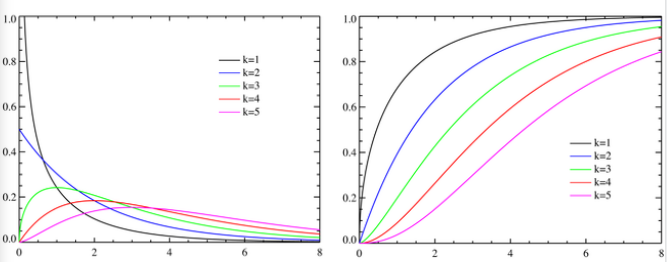
\includegraphics[scale=0.7]{img/chi.png}
\end{center}
\subsubsection{t di Student}
Siano $Z\sim N(0,1)$ e $Y\sim \chi_n^2$ due variabili indipendenti. Sia X una variabile aleatoria così definita:
\[X=\frac{Z}{\sqrt{\frac{Y}{n}}}\]
Una tale variabile è distribuita secondo una \textbf{t di student con n gradi di libertà}:
\[X\sim t_n\]
\textit{Questa distribuzione è di grande interesse come la distribuzione Normale e la distribuzione Chi-Quadro}.
\begin{center}
	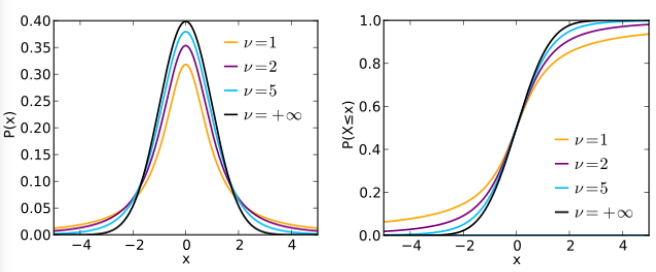
\includegraphics[scale=0.7]{img/t.png}
\end{center}
\subsubsection{Distribuzione F}
Siano $U\sim\chi_m^2$ e $V\sim\chi_n^2$ due variabili indipendenti. Sia X una variabile aleatoria così definita:
\[X=\frac{\frac{U}{m}}{\frac{V}{n}}\]
Una tale variabile è
distribuita secondo una \textbf{F con m ed n gradi di libertà}:
\[X\sim F(m,n)\]
\textit{Questa distribuzione è di grande interesse come la distribuzione Normale, la
distribuzione Chi-Quadro e la distribuzione t di Student}.
\begin{center}
	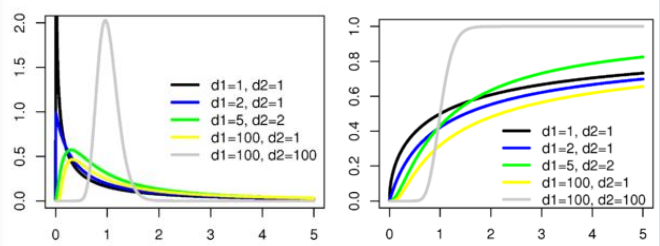
\includegraphics[scale=0.7]{img/f.png}
\end{center}
\end{document}
